% ==================== 3 原始数据整理与多曲线绘制 ====================
\section{原始数据整理与多曲线绘制}

课程课件把 XRD 数据的表示要求概括为四条：按科技论文规范绘图、能绘制多曲线图、能绘制含 PDF 卡片的多曲线图、能转换不同波长的数据\cite{shi2024xray}。本次作业对应前三条，下面从原始 txt 的格式问题开始。

\subsection{原始数据格式与两个 Origin 坑}

仪器导出的 txt 使用 GBK 编码，前 9 行是实验日期、文件路径、样品序号、实验者、起始角、终止角、步宽、波长和管压/管流等元数据，之后才是两列数据：第一列 $2\theta$（保留 4 位小数），第二列计数强度（整数）。图~\ref{fig:data}(a) 是 200.txt 的原始截图，可以看到元数据行和后面的数据行混在一起，真正的数据从第 10 行才开始。

原始文件看起来只是普通的空格分隔文本，但直接拖进 Origin 会碰到两个问题。第一个问题是分隔符：全文件唯一的英文逗号出现在 \texttt{0 kV, 0 mA} 这一行，Origin 的自动识别会据此把逗号当成列分隔符，而真正的数据行用空格分隔，结果整张表只剩一列。第二个问题是表头识别：Origin 的规则是字段数比数据行少的行归入 Main Header，之后头 3 个字段数与数据行相同的行依次当作列名、单位和备注。原始文件中的 \texttt{起始角= 20}、\texttt{终止角= 80}、\texttt{步宽= 0.02} 都只有两个字段，就被误认成了列名、单位和备注，真正的元数据反而落进数据区。图~\ref{fig:data}(b) 是直接导入后的结果：表头变成了 \texttt{0 kV}、\texttt{0 mA}，数据列也不对，显然不能直接用来画图。

\begin{figure}[H]
  \centering
  \begin{subfigure}[t]{0.32\textwidth}
    \centering
    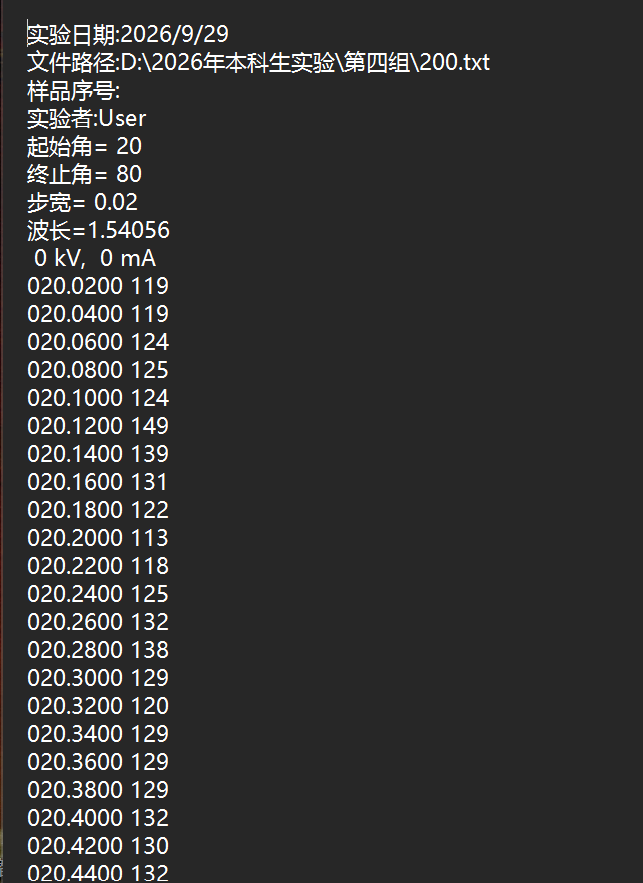
\includegraphics[width=\linewidth,height=5.0cm,keepaspectratio]{assets/origin/origin_data_raw.png}
    \caption{原始 200.txt}
  \end{subfigure}\hfill
  \begin{subfigure}[t]{0.32\textwidth}
    \centering
    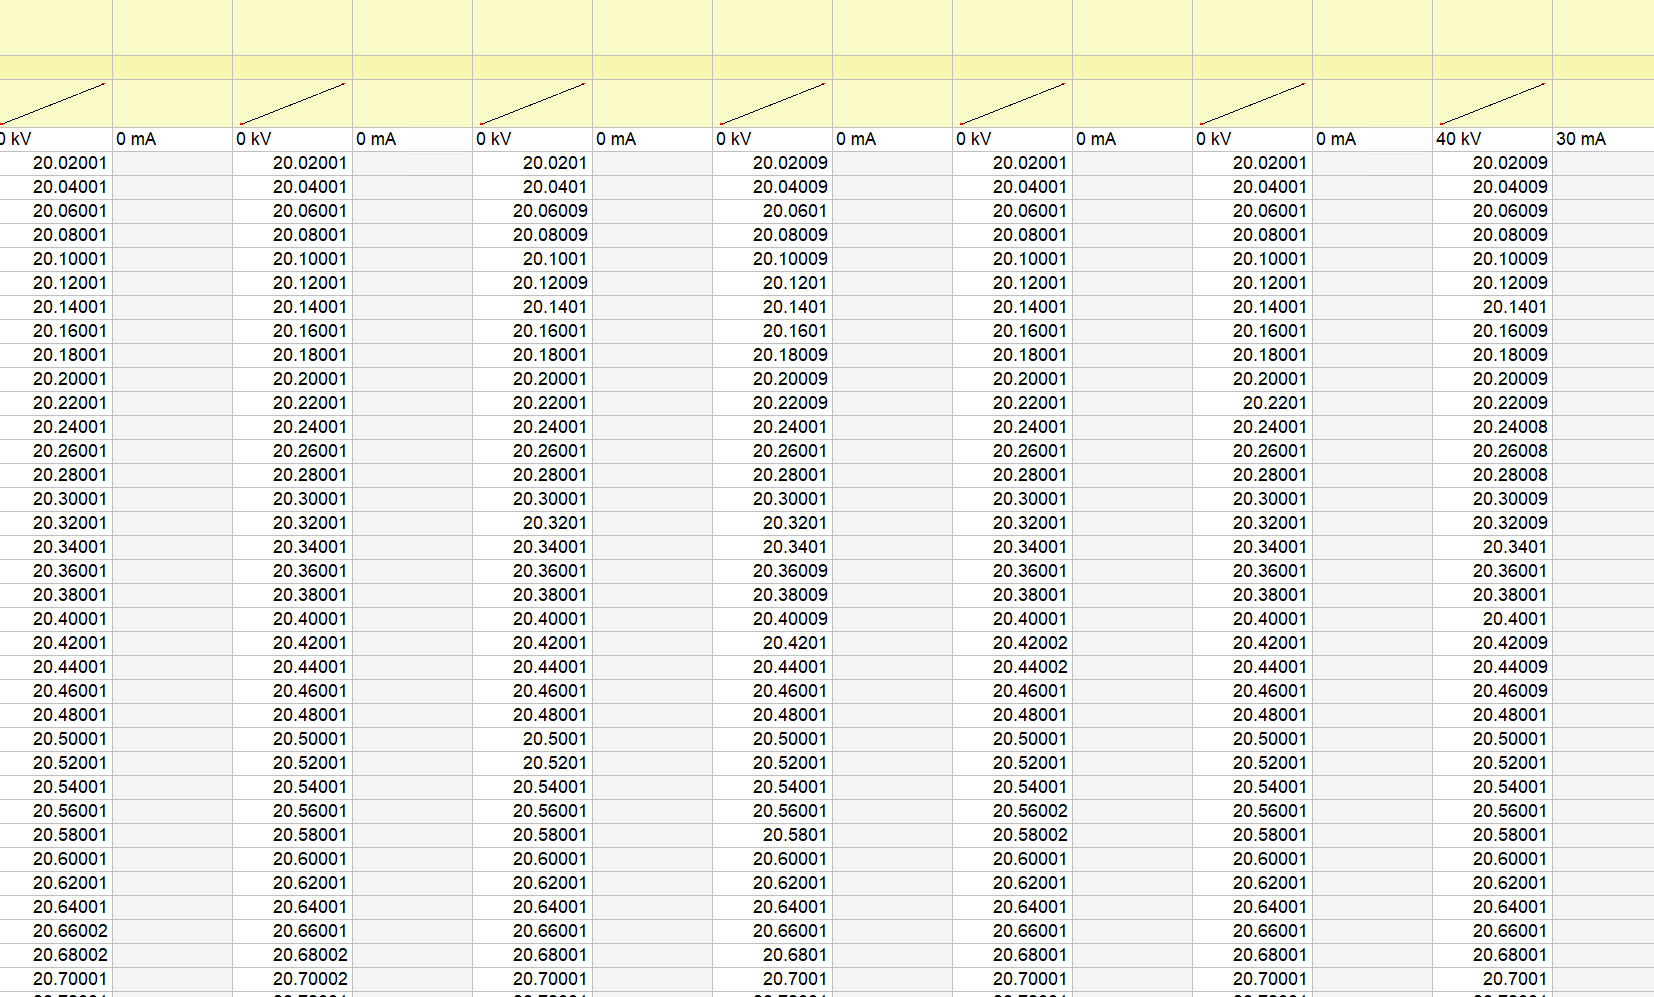
\includegraphics[width=\linewidth,height=5.0cm,keepaspectratio]{assets/origin/origin_data_wrong.png}
    \caption{直接导入 Origin 的结果}
  \end{subfigure}\hfill
  \begin{subfigure}[t]{0.32\textwidth}
    \centering
    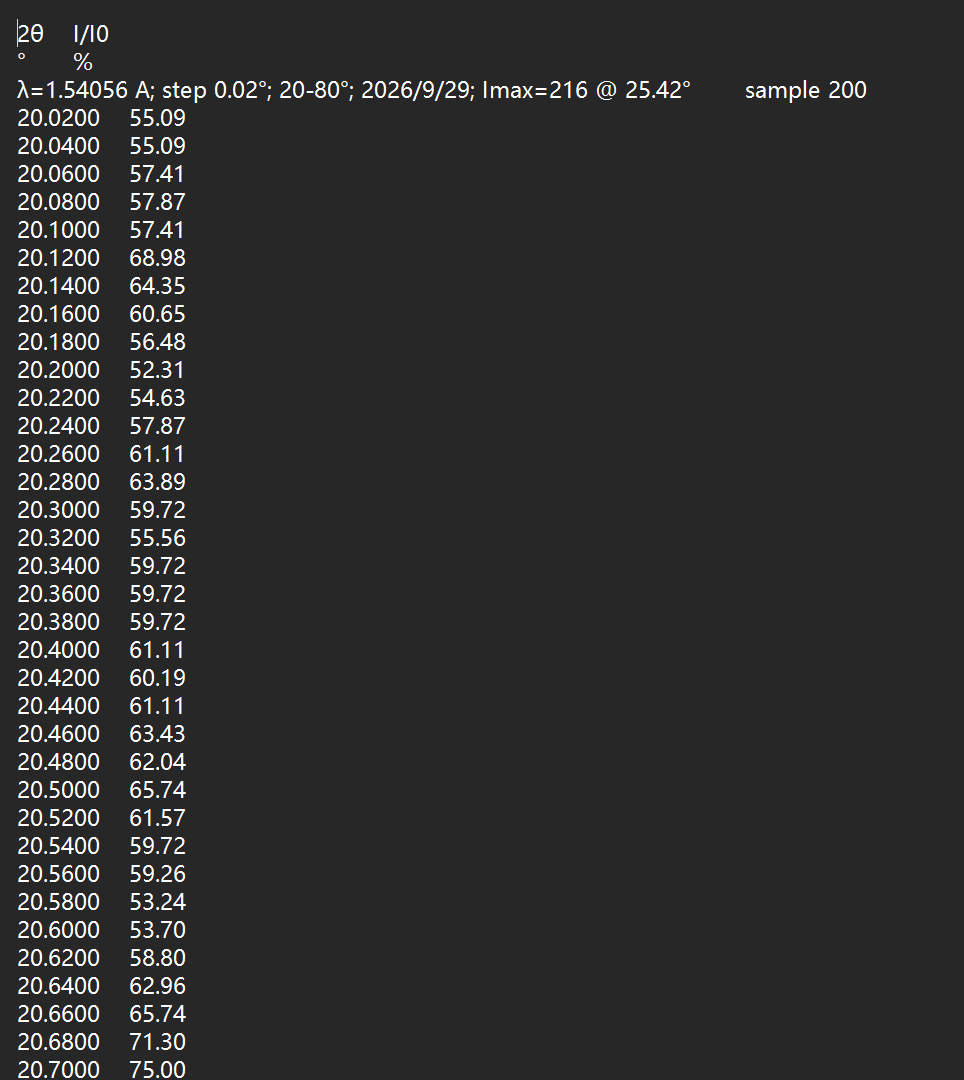
\includegraphics[width=\linewidth,height=5.0cm,keepaspectratio]{assets/origin/origin_data_norm.png}
    \caption{脚本转换并归一化后的数据}
  \end{subfigure}
  \caption{原始数据与脚本转换结果对比。(a) 仪器导出的 txt，前 9 行为元数据；(b) 直接导入 Origin 后表头错位、数据列不正确；(c) \texttt{make\_\allowbreak origin\_\allowbreak ready.py} 输出的 3 行表头 + Tab 分隔数据（已归一化）。}
  \label{fig:data}
\end{figure}

\subsection{用 make\_origin\_ready.py 转换 txt}

解决的办法不是手工删行，而是把文件重排成 Origin 能稳定识别的格式。自编脚本 \texttt{make\_\allowbreak origin\_\allowbreak ready.py} 只依赖 Python 标准库，把每个文件写成“3 行表头 + Tab 分隔的两列数据”，三行表头每行都严格两个字段，数据从第 4 行开始。在作业二根目录下运行

\begin{center}
\texttt{python .\textbackslash 脚本\textbackslash make\_origin\_ready.py 资料\textbackslash 原数据 --norm}
\end{center}

脚本会读取 \texttt{资料/原数据/} 下的 200.txt--900.txt，把原始强度写到 \texttt{ready/}，把归一化强度写到 \texttt{ready\_norm/}。输出文件的简化形式如下：

\begin{verbatim}
2theta    I/I0
degree    %
lambda=1.54056 A; step 0.02 deg; 20-80 deg; Imax=216 @ 25.42 deg    sample 200
20.0200    55.09
20.0400    55.09
\end{verbatim}

第一行对应 Origin 的 Long Name，第二行对应 Units，第三行对应 Comments；脚本把波长、步宽、角度范围、测试日期、最强峰位置和样品编号都塞进 Comments 行，既保留了元数据，又不会干扰列识别。归一化版本把每个样品的强度除以自己的最强峰再乘以 100，得到 $I/I_0$。这样处理之后，同一张图上的 8 条曲线峰高可比，但要注意每个样品是各自归一化的：跨样品比较绝对强度时不能直接用这张图，峰形和峰位比较则不受影响。图~\ref{fig:data}(c) 是转换后的 200.txt，表头和数据列都已经规整。

脚本对原始文件只读不写，输出写在 \texttt{资料/原数据/ready/} 和 \texttt{ready\_norm/} 两个新目录中；同样的内容也整理在 \texttt{资料/处理后数据/} 下，方便直接取用。转换后的 8 个文件命名保持不变（200.txt--900.txt），Comments 行里带有样品编号，导入 Origin 后不会混淆。

\subsection{Origin 中的多曲线绘制}

下面按实际操作顺序分成 6 步，每一步对应一张截图。这样写是为了让“点哪里、选什么”能和截图一一对上，而不是把 6 个操作挤在一段文字里。

\paragraph{步骤 1：打开 Multiple ASCII 导入}
在 Origin 中执行 \texttt{Data $\rightarrow$ Import from File $\rightarrow$ Multiple ASCII}，如图~\ref{fig:origin-step1}。

\begin{figure}[H]
  \centering
  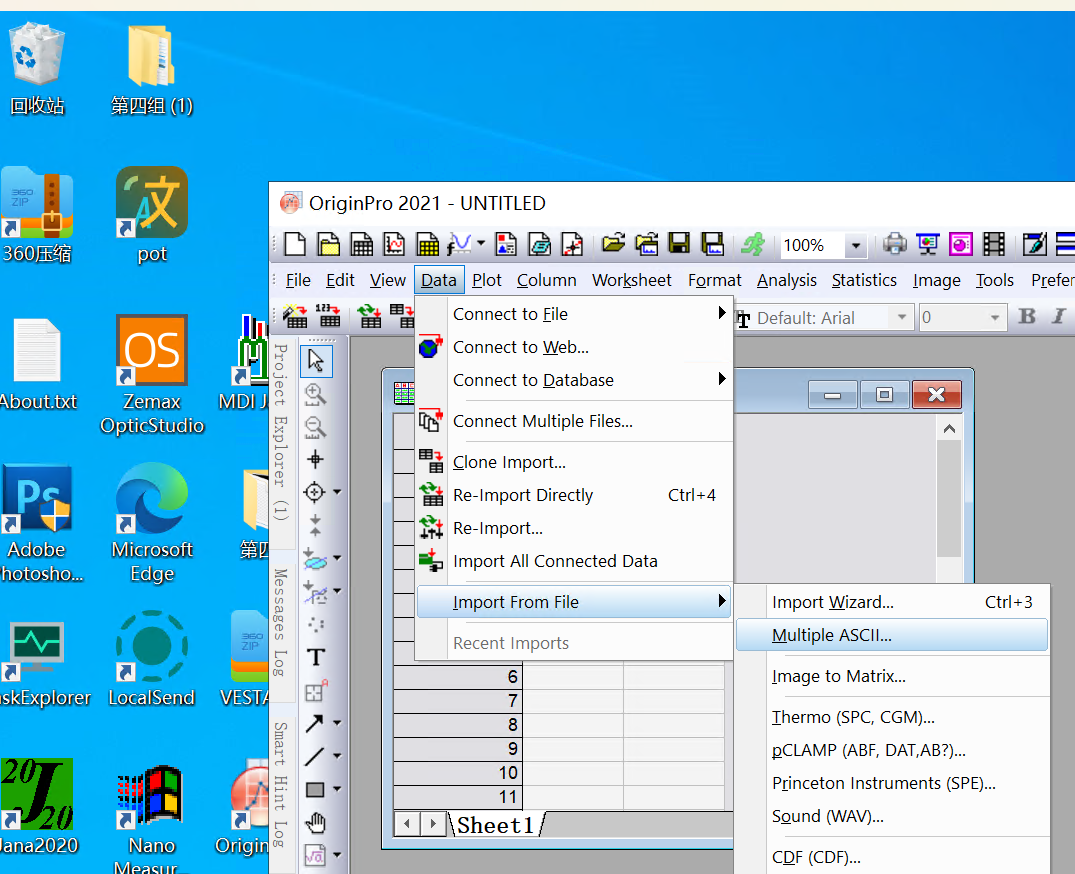
\includegraphics[width=\textwidth,height=6.5cm,keepaspectratio]{assets/origin/origin_01_import.png}
  \caption{步骤 1：Data $\rightarrow$ Import from File $\rightarrow$ Multiple ASCII。}
  \label{fig:origin-step1}
\end{figure}

\paragraph{步骤 2：选择 ready\_norm 文件夹}
在弹出的 ASCII 对话框中，把 Look in 选到 \texttt{资料/原数据/ready\_norm/}，如图~\ref{fig:origin-step2}。

\begin{figure}[H]
  \centering
  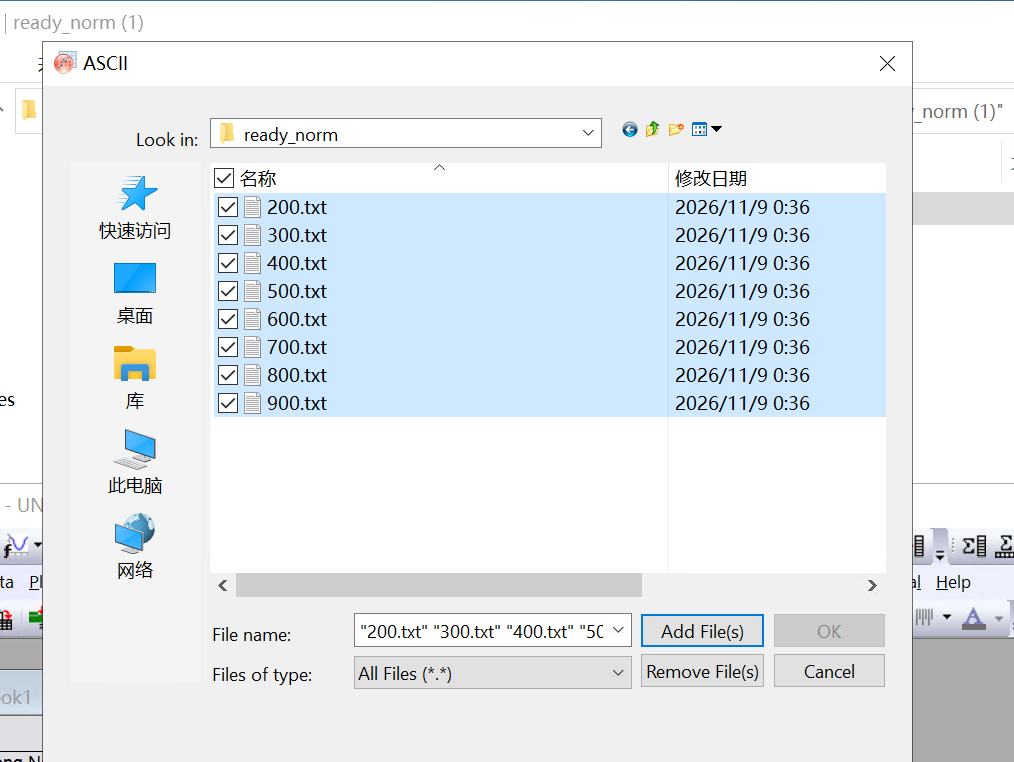
\includegraphics[width=\textwidth,height=6.5cm,keepaspectratio]{assets/origin/origin_select_folder.png}
  \caption{步骤 2：选择 ready\_norm 文件夹。}
  \label{fig:origin-step2}
\end{figure}

\paragraph{步骤 3：选中 200--900.txt}
在文件列表里选中 200.txt--900.txt，Files of type 选 \texttt{All Files (*.*)}，否则 txt 可能被过滤掉，如图~\ref{fig:origin-step3}。

\begin{figure}[H]
  \centering
  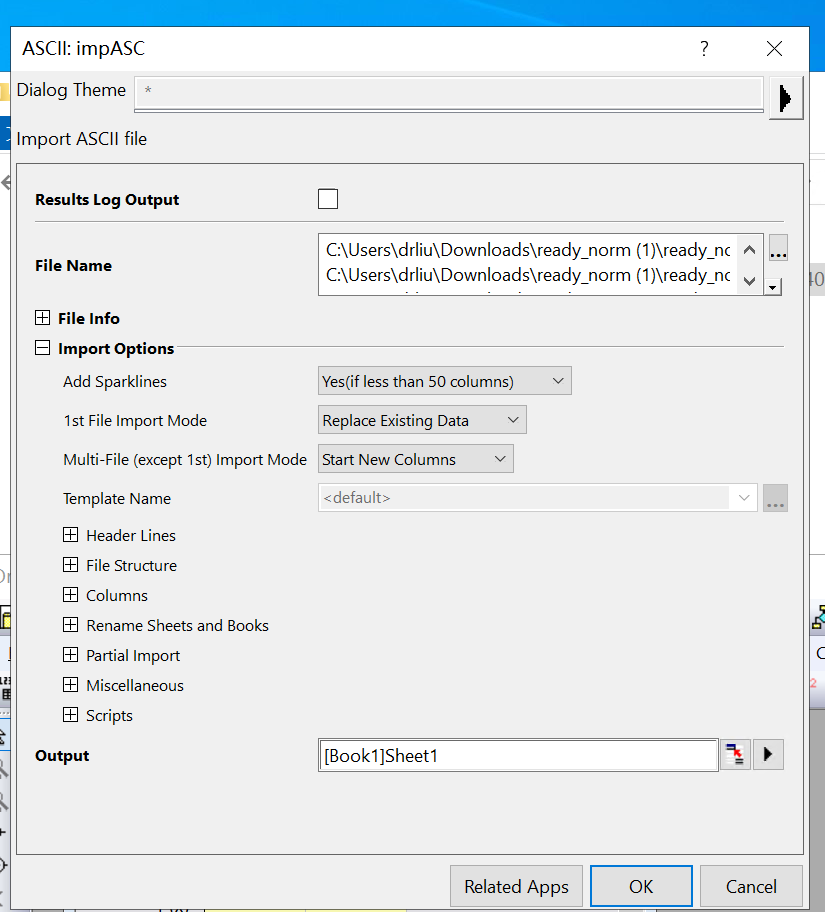
\includegraphics[width=\textwidth,height=6.5cm,keepaspectratio]{assets/origin/origin_select_txt.png}
  \caption{步骤 3：选中 200--900.txt（文件类型选 All Files）。}
  \label{fig:origin-step3}
\end{figure}

\paragraph{步骤 4：设置 Start New Columns}
在 Import Options 里，1st File Import Mode 选 \texttt{Start New Columns}；Multi-File (except 1st) Import Mode 也选 \texttt{Start New Columns}，这样 8 组数据会排在同一张工作表的不同列中。若选 \texttt{Start New Books}，每组会进入新工作簿，后续还要合并，如图~\ref{fig:origin-step4}。

\begin{figure}[H]
  \centering
  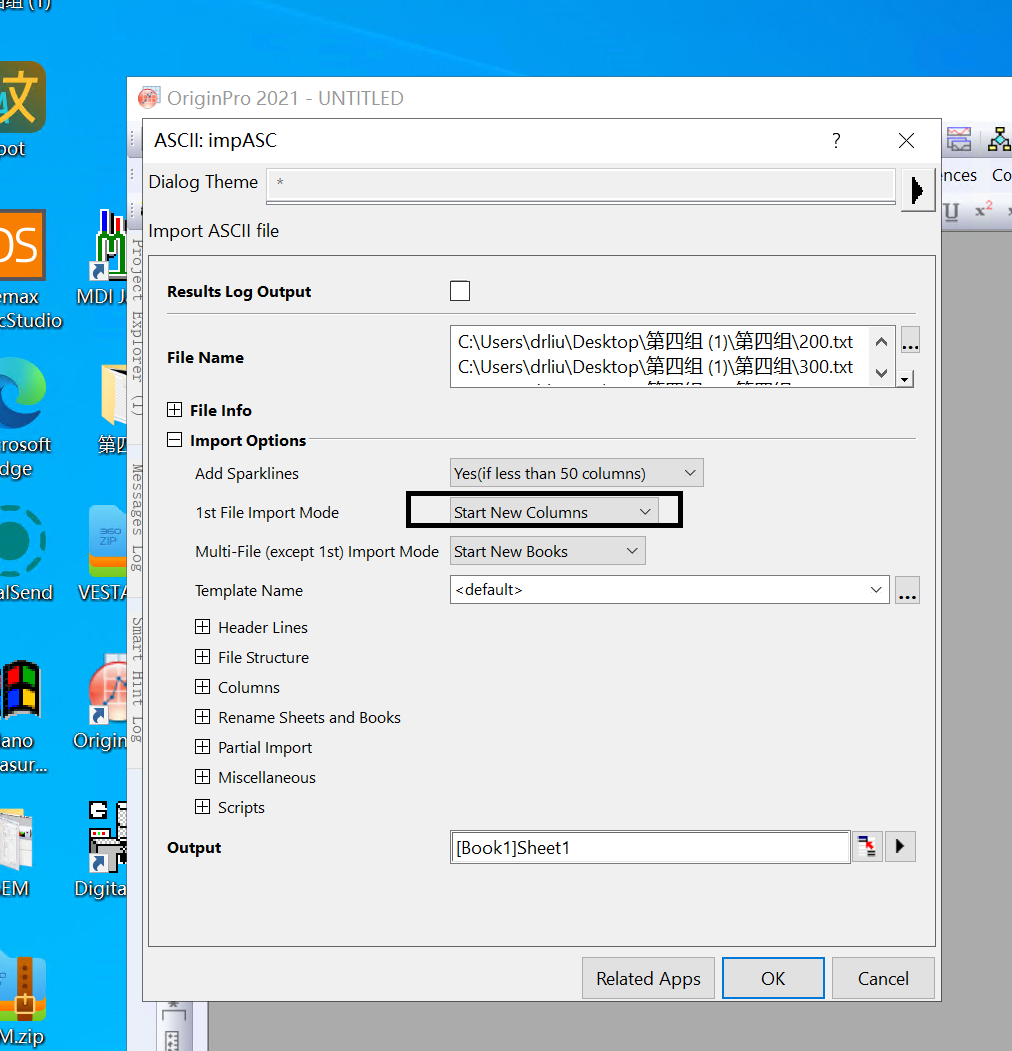
\includegraphics[width=\textwidth,height=6.5cm,keepaspectratio]{assets/origin/origin_02_new_columns.png}
  \caption{步骤 4：第一个文件用 Start New Columns；多文件模式也选 Start New Columns。}
  \label{fig:origin-step4}
\end{figure}

\paragraph{步骤 5：Stacked Lines by Y Offsets}
导入后，把每组的第一列 Set As X、第二列 Set As Y；选中 8 组 Y 列，执行 \texttt{Plot $\rightarrow$ Stacked Lines by Y Offsets}，如图~\ref{fig:origin-step5}。

\begin{figure}[H]
  \centering
  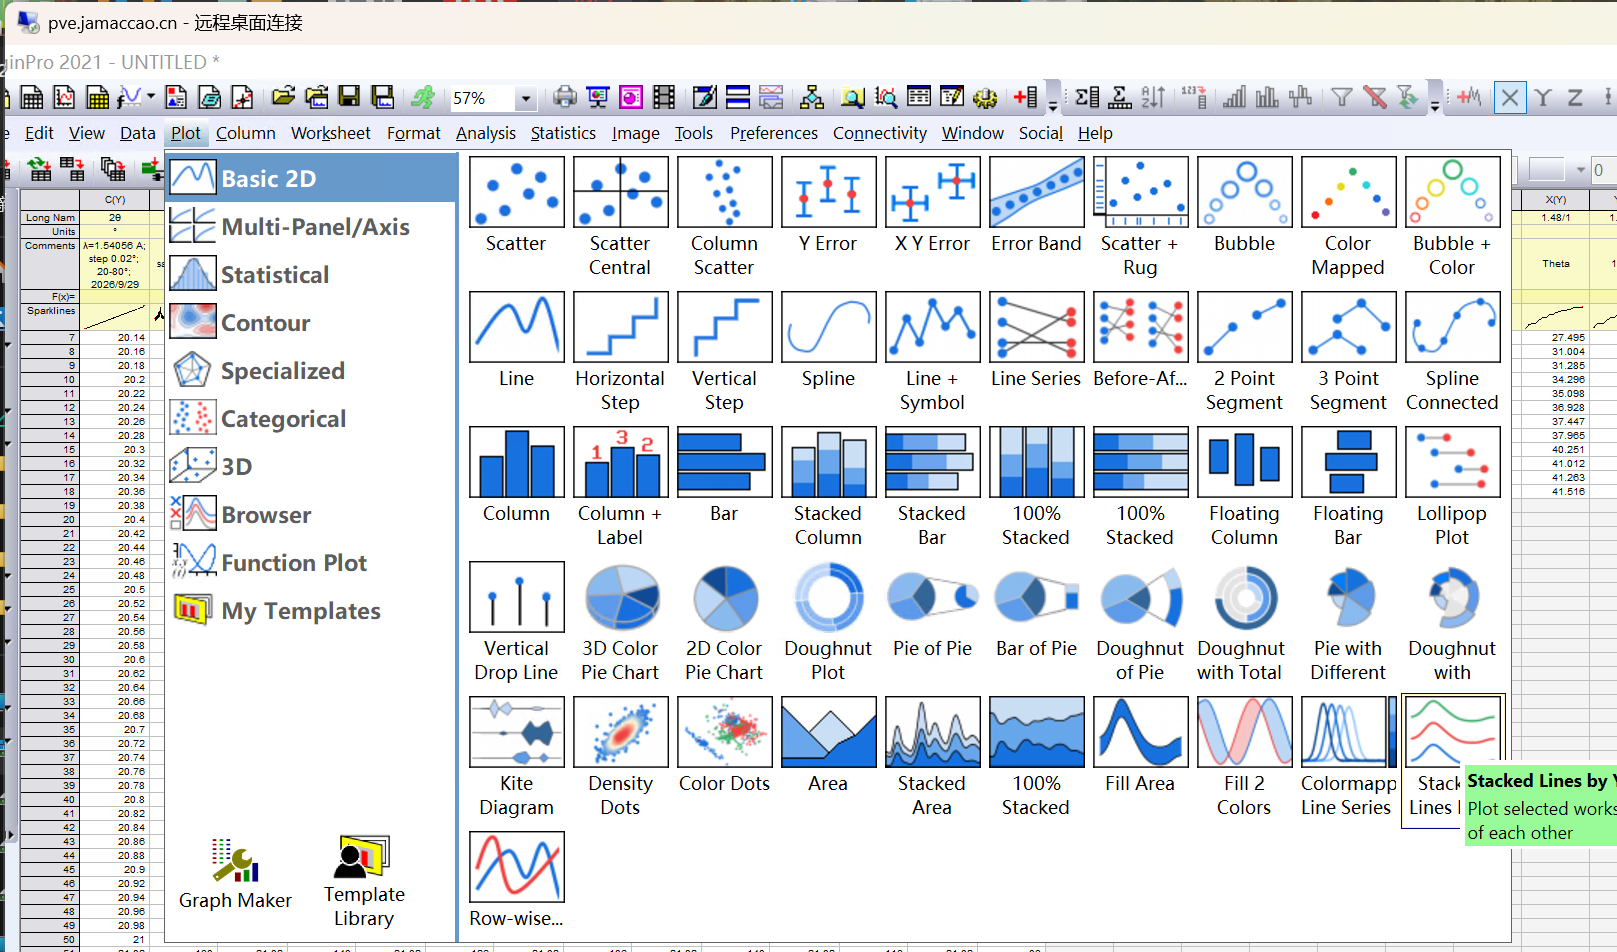
\includegraphics[width=\textwidth,height=6.5cm,keepaspectratio]{assets/origin/origin_03_stacked.png}
  \caption{步骤 5：Plot $\rightarrow$ Stacked Lines by Y Offsets。}
  \label{fig:origin-step5}
\end{figure}

\paragraph{步骤 6：得到叠图并统一格式}
Origin 按 Y 偏移把 8 条曲线错开，结果如图~\ref{fig:origin-step6}。接下来统一坐标轴：$2\theta$ 范围 20--80$^\circ$，主刻度 10$^\circ$、次刻度 2$^\circ$；Y 轴只保留 “Intensity (a.u.)” 的轴标题，不显示具体刻度。图例、线宽和字体按科技论文的惯例设置，导出 600 dpi PNG 或矢量 PDF，不要用屏幕截图——课程课件中明确要求“在正式场合绝对不允许拷屏，需用 Origin 等专业绘图软件画图”\cite{shi2024xray}。

\begin{figure}[H]
  \centering
  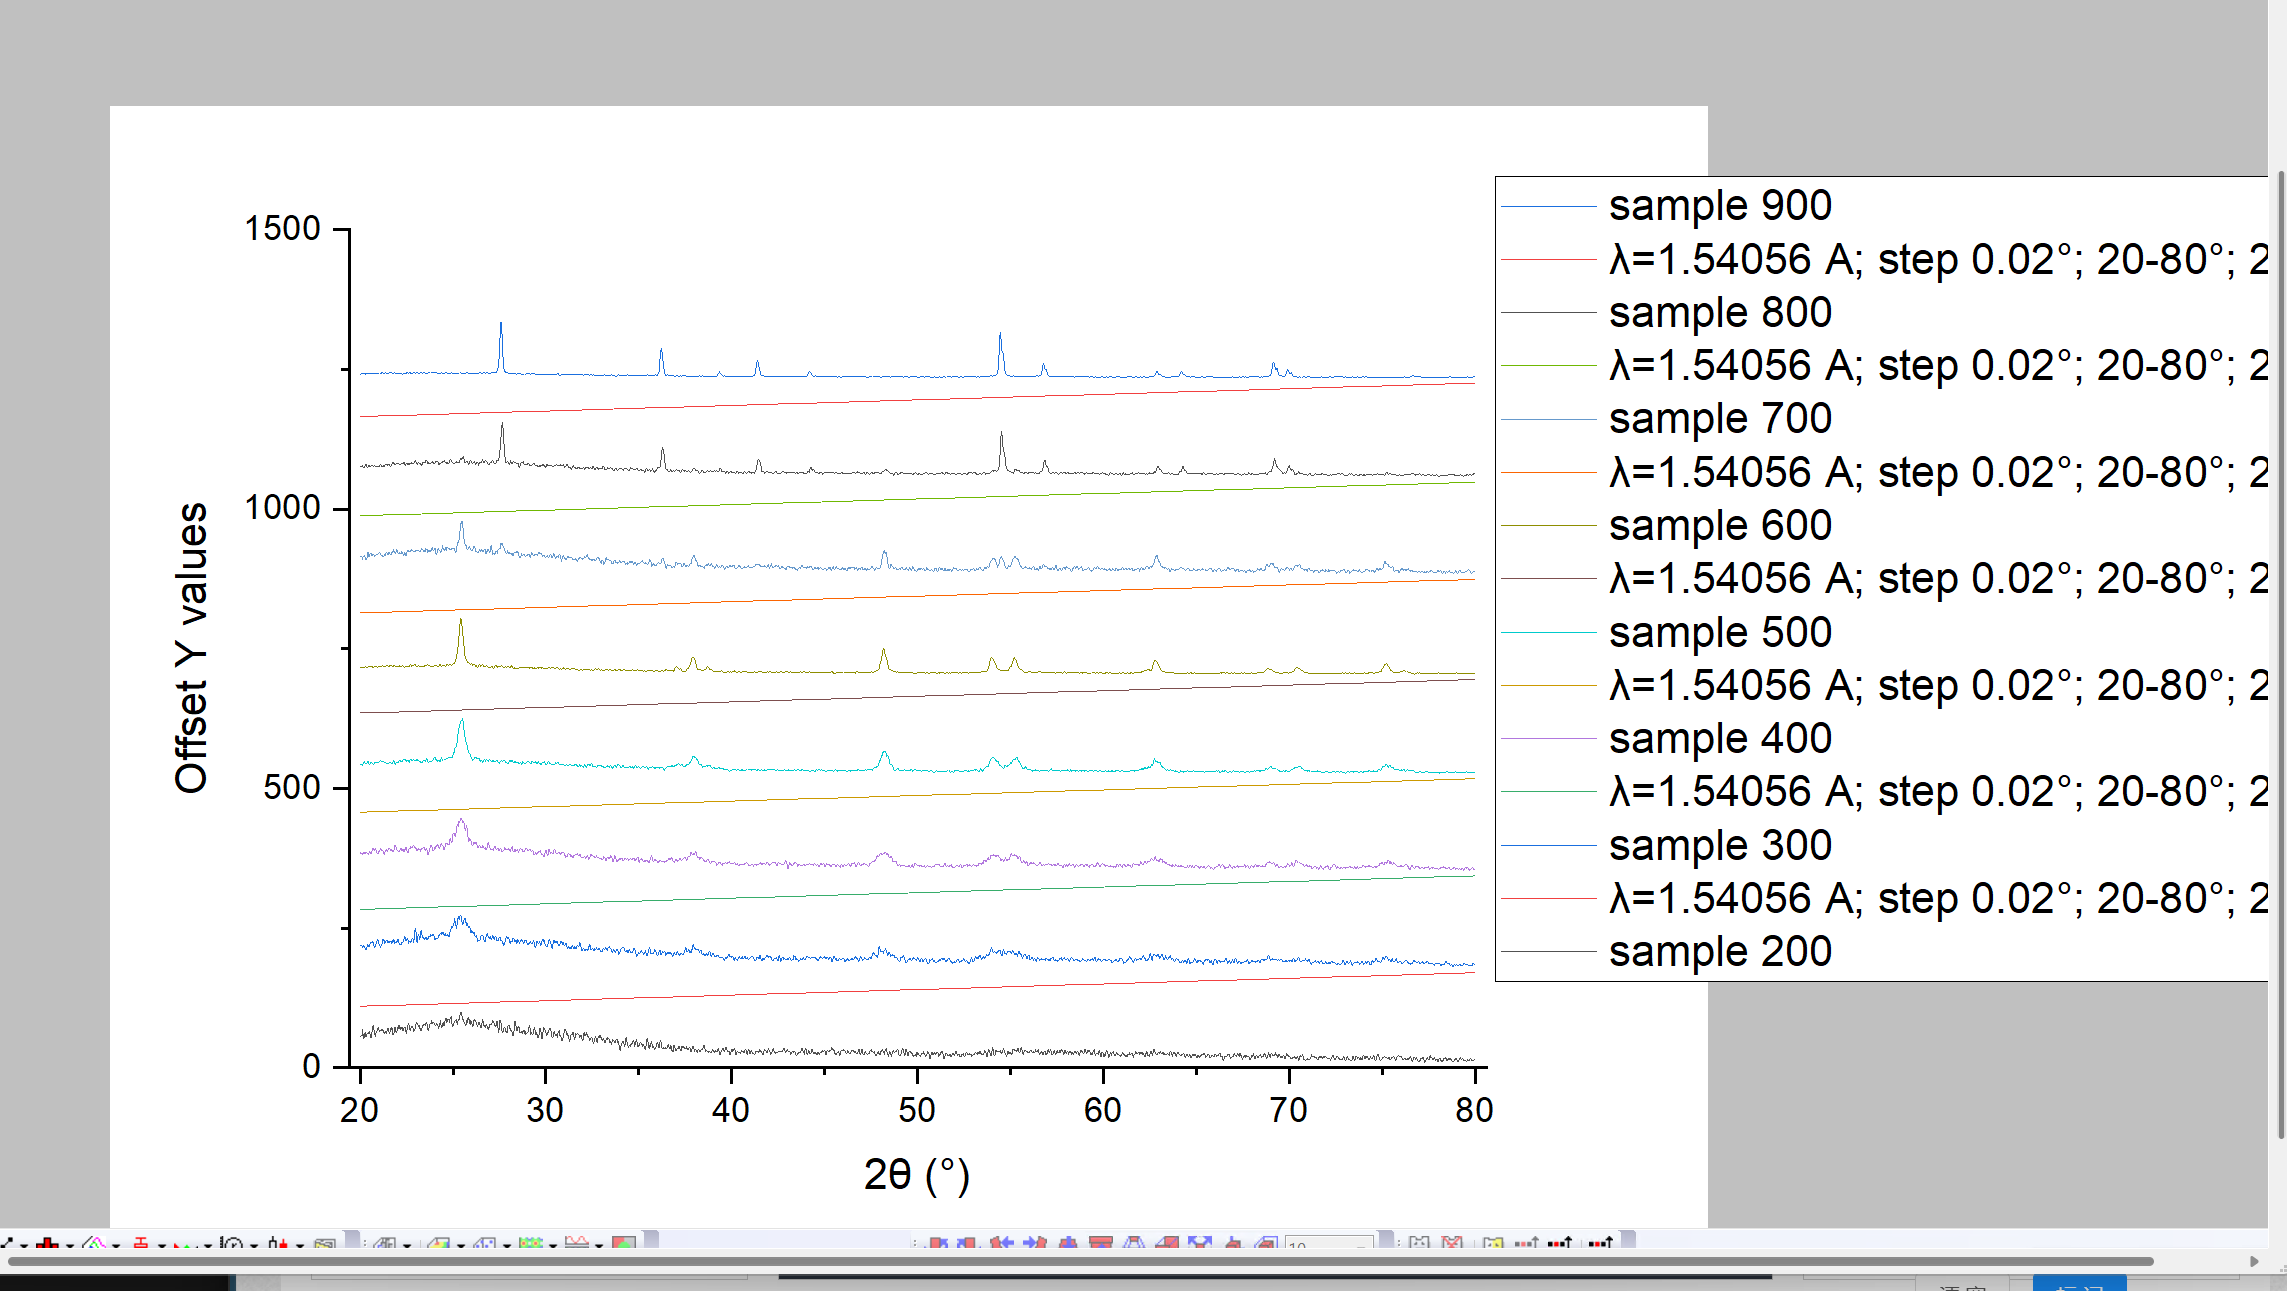
\includegraphics[width=\textwidth,height=6.5cm,keepaspectratio]{assets/origin/origin_stacked_result.png}
  \caption{步骤 6：Origin 叠图结果。}
  \label{fig:origin-step6}
\end{figure}

\subsection{数据整理与快速核对}

8 组原始数据的文件都在 \texttt{资料/原数据/}，转换后的文件在 \texttt{ready/} 和 \texttt{ready\_norm/}，最终画图用的成品在 \texttt{资料/处理后数据/}。表~\ref{tab:data} 列出了每组原始数据的最强峰位置和定性物相，用来快速核对“哪一组该出现哪个峰”。表中的峰位是原始数据最大值所在的位置，只用于快速判断，不是精确峰位；精确的峰位对照放在第 4 节结合 PDF 卡片做。

\begin{table}[H]
  \centering
  \caption{8 组样品的原始最强峰与定性物相}
  \label{tab:data}
  \small
  \begin{tabular}{@{}cccc@{}}
    \toprule
    样品 & 原始最强峰/计数 & 峰位/$^\circ$ & 定性物相 \\
    \midrule
    200 & 216  & 25.42 & 锐钛矿（宽包，结晶度低） \\
    300 & 289  & 25.38 & 锐钛矿 \\
    400 & 344  & 25.42 & 锐钛矿 \\
    500 & 544  & 25.50 & 锐钛矿 \\
    600 & 766  & 25.42 & 锐钛矿 \\
    700 & 347  & 25.48 & 锐钛矿（开始出现金红石） \\
    800 & 557  & 27.66 & 金红石为主，少量锐钛矿 \\
    900 & 1328 & 27.58 & 金红石 \\
    \bottomrule
  \end{tabular}
  \par\vspace{3pt}
  {\footnotesize 注：峰位为原始数据最大值位置，仅用于快速核对；精确峰位需结合 PDF 卡片逐峰对照。}
\end{table}
